\begin{figure*}[t]
\centering
% Vector drawing generated by tools/figures/lookup.py; rerun it after changing the figure.
\ifbilingual
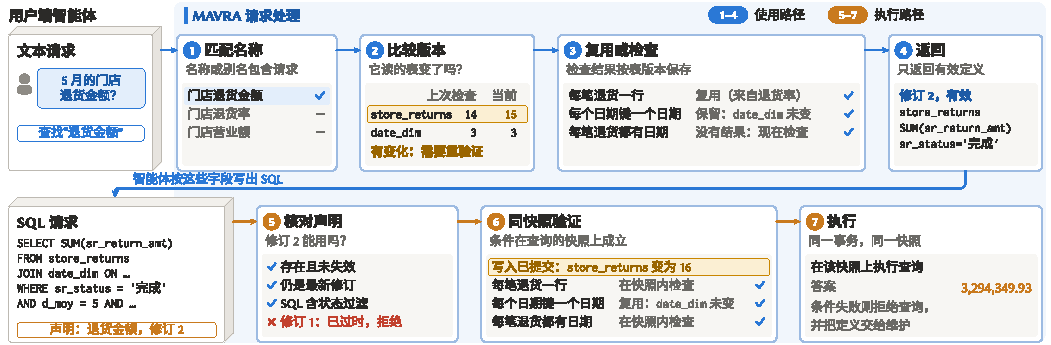
\includegraphics[width=\textwidth]{figures/lookup-zh}
\else
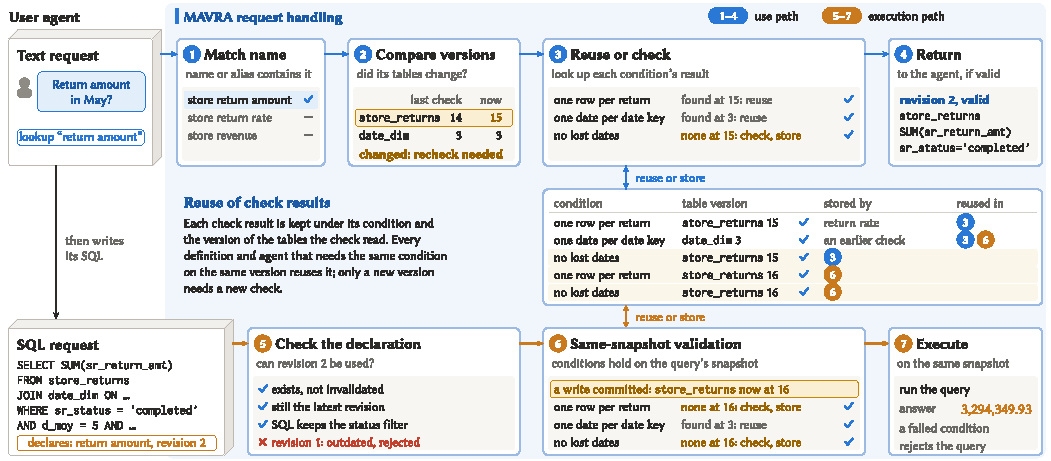
\includegraphics[width=\textwidth]{figures/lookup}
\fi
\caption{\bt{Request handling by example, for revision 2 of the return-amount definition, the repaired revision of Figure~\ref{fig:lifecycle}. Check results (middle) are kept per condition and table version and shared by all definitions and agents: lookup reuses a result that the return-rate definition stored (3), and a write between lookup and query makes validation check two conditions inside the query's snapshot and store their results for later requests (6).}{请求处理示例，所用定义为退货金额的修订 2，即图~\ref{fig:lifecycle} 中修复后的修订。检查结果（中间）按“条件 + 表版本”保存，所有定义与智能体共用：查找复用退货率定义存入的结果（3）；查找与查询之间有一次写入，所以验证在查询的快照内检查两个条件，并存入结果供之后的请求复用（6）。}}
\label{fig:lookup}
\Description{Two lanes of steps with a table of check results between them. Top lane, the use path: a user agent asks for the return amount in May and looks up ``return amount''. Step 1 matches names and aliases: store return amount matches, store return rate and store revenue do not. Step 2 compares versions: store\_returns was at version 14 at the last check and is now at 15, date\_dim is at 3 both times, so the definition must be rechecked. Step 3 looks up each condition's result: one row per return is found at version 15 and reused, one date per date key is found at version 3 and reused, and no lost dates has no result at 15, so it is checked and stored. Step 4 returns revision 2 as valid, with the table store\_returns, the measure SUM(sr\_return\_amt), and the filter sr\_status = 'completed'. The middle table lists the check results with condition, table version, who stored each one, and which step reused it: one row per return at store\_returns 15, stored for return rate and reused in step 3; one date per date key at date\_dim 3, stored by an earlier check and reused in steps 3 and 6; no lost dates at 15, stored in step 3; one row per return and no lost dates at 16, stored in step 6. A note beside it explains that a result is kept under its condition and the version of the tables it read, and every definition and agent that needs the same condition on the same version reuses it. Bottom lane, the execution path: the agent then writes SQL that sums sr\_return\_amt over completed returns in May and declares return amount, revision 2. Step 5 checks that the revision exists, is not invalidated, is still the latest, and that the SQL keeps the status filter; revision 1 would be rejected as outdated. Step 6 validates on the query's snapshot, in which a write has committed so that store\_returns is at version 16: the two conditions on store\_returns are checked and stored, and the date condition is reused. Step 7 runs the query on the same snapshot and returns 3,294,349.93; a failed condition would reject the query.}
\end{figure*}
